
\documentclass[12pt]{article}

\usepackage[a4paper]{geometry}
\usepackage{cmap} %for right cyrillic encoding in PDF files
\usepackage[T2A]{fontenc}
\usepackage[utf8]{inputenc}
\usepackage[russian]{babel}
\usepackage{graphicx}
\usepackage{color}
\usepackage[unicode=true,pdfborder={0 0 0}]{hyperref}
\usepackage{caption}
\usepackage{amssymb,amsmath}
\usepackage{mathtext}
\usepackage{xspace}
\usepackage{hyperref}

\input{/home/skononov/tex/defs}
\input{/home/skononov/tex/tabledefs}

\textheight 23cm
\textwidth 16cm
\topmargin 0cm
\oddsidemargin -.5cm
\footskip 1.5cm

\newcommand{\lsc}{\ensuremath{L_\mathrm{sc}}\xspace}
\newcommand{\betaop}{\ensuremath{\beta_\mathrm{0}}\xspace}

\title{\Large\bf Меморандум по оптимизации радиатора ФАРИЧ}
\author{\large н.с. лаб. 3-2 Кононов С.А.}
\date{\large 01.11.2018 г.}

\begin{document}
\maketitle

\section{Расчет разрешения ФАРИЧ}
\subsection{Теория}
Число черенковских фотонов на единицу длины волны излучения и единицу пути частицы в среде (радиаторе):
\begin{equation}
\frac{d^2N}{dx d\lambda} = \frac{2\pi\alpha z^2}{\lambda^2}\left(1 - \frac{1}{\beta^2 n^2(\lambda)}\right),
\label{eq:cherint}
\end{equation}
где $x$ -- координата вдоль пути частицы, $\lambda$ -- длина волны излучения,
$n(\lambda)$ -- показатель преломления в среде с дисперсией,
$\beta$ -- скорость частицы в единицах скорости света в вакууме $c$, $z$ -- заряд частицы в единицах элементарного заряда, 
$\alpha\approx 1/137$ -- постоянная тонкой структуры.

Формулу (\ref{eq:cherint}) можно также использовать для неоднородной среды, которой является аэрогелевый радиатор детектора ФАРИЧ, вводя
зависимость показателя преломления от координаты вдоль пути частицы $n(x,\lambda)$.

Для фотонного детектора с эффективностью регистрации $\mathrm{PDE}(\lambda)$ и радиатора с коэффициентом сбора 
фотонов $\mathrm{LC}(x,\lambda)$ число зарегистрированных фотонов равно:
\begin{equation}
\frac{d^2N_\mathrm{pe}}{dx d\lambda} = \frac{2\pi\alpha z^2}{\lambda^2}\left(1 - \frac{1}{\beta^2 n^2(x,\lambda)}\right)
\mathrm{PDE}(\lambda)\mathrm{LC}(x,\lambda).
\label{eq:cherintdet}
\end{equation}

В данной работе расчет разрешения детектора ФАРИЧ производится в случае, когда радиатор представляет из себя множество непосредственно граничащих между 
собой плоскопараллельных слоев аэрогеля диоксида кремния, расположенных перпендикулярно направлению движения частицы. Слои аэрогеля характеризуются своей 
толщиной и показателем преломления. Поглощение фотонов --- одинаковое для всех слоев и определяется только длиной пути фотона в радиаторе и длиной поглощения. 
Рэлеевское рассеяние фотонов в аэрогеле считается эквивалентным поглощению, 
так как при этом теряется информация о направлении излучения фотона, а фоном, который создается рассеянными фотонами от одной частицы можно пренебречь в практически важных случаях. 
Плоскость входного окна координатно-чувствительного фотонного детектора расположена параллельно плоскости радиатора на некотором расстоянии от радиатора. 
Между радиатором и фотонным детектором расположена абсолютно прозрачная среда с показателем преломления равным единице (``воздух''). 
В этом случае черенковские фотоны создают распределение в плоскости входного окна фотонного детектора в форме колец или кольца с центром 
совпадающим с точкой пересечения частицы и входного окна фотонного дететора. 
В работе рассматривается вариант однокольцевого детектора ФАРИЧ, когда показатели преломления и толщины 
слоев аэрогеля для некоторой заданной скорости частицы подбираются такими, чтобы распределения фотонов в плоскости фотонного 
детектора от каждого слоя совпадали наилучшим образом. На рисунке~\ref{fig:farich} для наглядности показана схема детектора ФАРИЧ с 
используемыми координатами и обозначениями.

\begin{figure}[htb]
\begin{center}
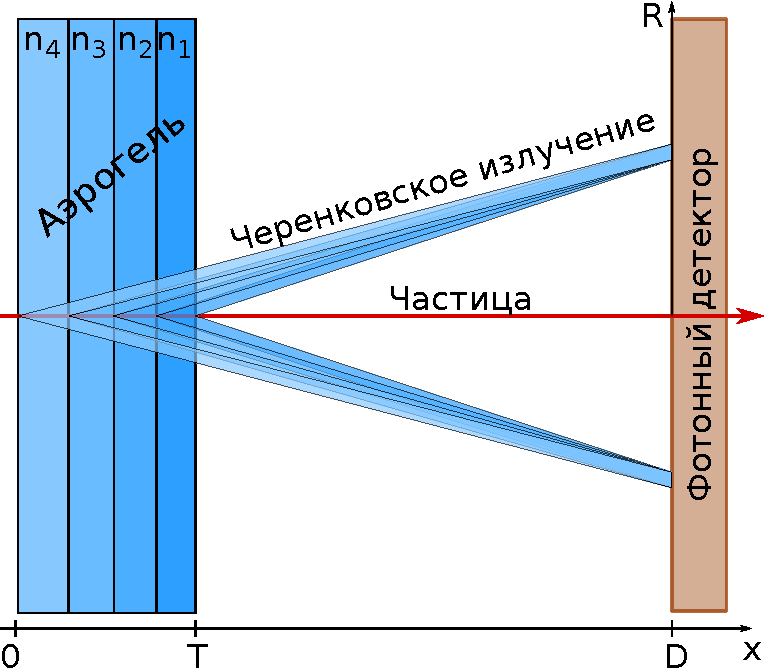
\includegraphics[width=0.4\textheight]{farich_scheme.pdf}
\caption{\small Схема детектора ФАРИЧ с четырьмя слоями аэрогеля.}
\label{fig:farich}
\end{center}
\end{figure}

Для расчета необходимо определить на какой радиус $R$ в плоскости фотонного детектора приходят фотоны с длиной волны $\lambda$, излученные в точке $x_0$ вдоль пути частицы в
радиаторе. Для этого необходимо проинтегрировать приращения радиуса фотонов при изменении координаты $x$ фотона от $x_0$ до попадания в фотонный детектор ($x=D$). В результате
получим
\begin{equation}
R(x_0,\lambda) = \int_{x_0}^D \tan\psi(x_0,x;\lambda) dx,
\label{eq:rx0psi}
\end{equation}
где $\psi(x_0,x;\lambda)$ -- это угол между направлением частицы и фотоном в точке с координатой $x$, который излучен в точке $x_0$. 
Угол $\psi$ в точке излучения фотона всегда равен черенковскому углу 
$\psi(x_0,x_0;\lambda) \equiv \theta_c(x_0,\lambda) = \arccos{1/n(x_0,\lambda)\beta}$, а в любой другой точке его можно определить из закона преломления Снелля:
\[n(x_0,\lambda)\sin\psi(x_0,x_0;\lambda) = n(x,\lambda)\sin\psi(x_0,x;\lambda).\]

В итоге можно получить выражение для тангенса угла $\psi$:
\begin{equation}
\tan\psi(x_0,x;\lambda) = \sqrt{\frac{n^2(x_0,\lambda)\beta^2-1}{(n^2(x,\lambda)-n^2(x_0,\lambda))\beta^2+1}},
\label{eq:tanpsi}
\end{equation}

Подставляя (\ref{eq:tanpsi}) в (\ref{eq:rx0psi}), получаем что радиус фотона в плоскости фотонного детектора равен
\begin{equation}
R(x_0,\lambda) = (D-T)\sqrt{\frac{n(x_0,\lambda)\beta^2-1}{(1-n^2(x_0,\lambda))\beta^2+1}} + 
\int_{x_0}^T \sqrt{\frac{n(x_0,\lambda)\beta^2-1}{n^2(x,\lambda)\beta^2-n^2(x_0,\lambda)\beta^2+1}} dx,
\label{eq:rx0}
\end{equation}

В расчете используется дисперсия показателя преломления, измеренная в работе \cite{aerdisp} для 
образца новосибирского аэрогеля, где показатель преломления в зависимости от длины волны описывается уравнением
\[n^2(\lambda)-1 = \frac{a_0 \lambda^2}{\lambda^2-\lambda_0^2},\]
где $a_0 = 0.05639$, $\lambda_0 = 83.22\,\textrm{нм}$. 
Для расчета аэрогелей с иной плотностью зависимость показателя преломления получается соответствующим изменением 
коэффициента $a_0$.

Расчет учитывает потерю прямого света из-за эффекта рэлеевского рассеяния, которое определяется длиной рассеяния $L_\textrm{sc}(\lambda)$.
Типовая длина рассеяния для новосибирского аэрогеля составляет 50\,мм при длине волны 400\,нм. Далее везде в расчетах используется это значение. 
Поглощением света в аэрогеле детектора черенковских колец можно пренебречь по сравнению потерями прямого света за счет рассеяния. Существуют также потери
прямого света при рассеянии на выходной поверхности аэрогеля, составляющие 2--5\% и независящие от длины волны.
Коэффициент светосбора $\mathrm{LC}$ в уравнении (\ref{eq:cherintdet}) в случае ФАРИЧ можно записать как \cite{aerscat}:
\[\mathrm{LC}(x_0,\lambda) = A \exp\left(-\frac{s(x_0,\lambda)}{L_\textrm{sc}(400\,\textrm{нм})\left(\lambda / 400\,\textrm{нм}\right)^4}\right),\]
где $A$ -- коэффициент рассеяния на выходной поверхности аэрогеля, $s(x_0,\lambda)$ -- длина пути фотона с длиной волны $\lambda$, 
возникающего в точке $x_0$, в радиаторе, которую можно найти с помощью интеграла:
\begin{equation}
s(x_0,\lambda) = \int_{x_0}^T \sqrt{1+\tan^2\psi(x_0,x;\lambda)} dx.
\label{eq:path}
\end{equation}

Для многослойного радиатора интегралы в (\ref{eq:tanpsi}), (\ref{eq:rx0}) и (\ref{eq:path}), очевидно, можно записать в виде соответствующих сумм по слоям радиатора, 
что опускается здесь.

Проинтегрировав по длине волны выражение (\ref{eq:cherintdet}), произведя замену переменной $x_0\to R$, можно получить искомое распределение числа фотоэлектронов по радиусу:
\begin{equation}
\frac{dN_\mathrm{pe}}{dR}(R) = \int_{\lambda_1}^{\lambda_2} d\lambda \sum_i \frac{d^2N_\mathrm{pe}}{dx d\lambda}(x_i(\lambda),\lambda)
\left|\frac{\partial R}{\partial x}(x_i(\lambda),\lambda)\right|^{-1},
\label{eq:dnpedr}
\end{equation}
где $\lambda_1,\,\lambda_2$ -- регистрируемый фотонным детектором диапазон длин волн, $x_i(\lambda)$ --- корни уравнения 
\[R(x,\lambda)=R\] 
по $x$ для соответствующей $\lambda$, то есть все точки вдоль пути частицы в радиаторе, из которых фотоны с длиной волны 
$\lambda$ попадают на радиус $R$. В случае многослойного радиатора из уравнения (\ref{eq:rx0psi}) следует
\[\frac{\partial R}{\partial x}(x,\lambda) = \tan\psi(x,x;\lambda).\]
Очевидно, что частные производные $\frac{\partial R}{\partial x}$ являются ненулевыми, а их обратные значения, входящие в (\ref{eq:dnpedr}), конечные. 

Средний радиус кольца и стандартная ошибка радиуса на один фотон $\sigma_1(R)$ находится известными методами теории вероятности из распределения (\ref{eq:dnpedr}).

Также полезно вычислить стандартные ошибки по углу $\theta$, задаваемым выражением 
\(\tan\theta = \frac{R}{D_{1/2}},\)
где $R$ -- радиус фотонов, $D_{1/2}$ -- расстояние от срединной плоскости радиатора до фотонного детектора.
В силу того, что показатель преломления аэрогеля в практике близок к 1, а, значит, изменение направления фотонов на границах сред небольшое, то 
угол $\theta$ близок по величине к черенковскому углу. Его можно назвать эффективным черенковским углом радиатора. Его величина для данного радиатора и фотонного детектора
зависит только от скорости частицы. Разрешение по углу $\theta$ (угловое разрешение) можно использовать для сравнения разных детекторов ФАРИЧ с фиксированным максимальным 
показателем преломления аэрогеля, в частности для оптимизации детектора ФАРИЧ по угловому разрешению.
Ошибка по углу, $\sigma(\theta)$, определяется из ошибки по радиусу $\sigma(R)$ методом переноса ошибок:
\[\sigma(\theta) = \frac{\sigma(R) D_{1/2}}{D_{1/2}^2+R^2}.\]

\subsubsection*{Расчет ошибки среднего радиуса на частицу}
Наилучшая оценка радиуса черенковского кольца на одну частицу есть арифметическое среднее радиусов фотонов, зарегистрированных в событии с одной частицей. 
Для оценки ошибки среднего требуется учесть, что число фотонов случайно меняется от события к событию. Предполагаем, что число фотонов
распределено по закону Пуассона и все радиусы фотонов независимо распределены с одинаковой функцией распределения. Для нулевого числа фотонов 
измерение, естественно, не производится, что следует учесть при расчете ошибки. 
В этом случае  можно вывести точную формулу для стандартной ошибки среднего радиуса на частицу (событие).
Будем исходить из известной формулы для дисперсии эмпирического среднего по математической выборке $(R_1, R_2, \ldots, R_N)$:
\[\displaystyle D(\bar{R}) = D\left(\frac{\sum_i R_i}{N}\right) = \frac{D(R_1)}{N}.\]

Далее возьмем математическое ожидание данного выражения для пуассоновской величины $N$ со средним $\nu$, исключая из пуассоновского распределения
значение $N=0$:
\[
E\left(\frac{D(R_1)}{N}\right) = \frac{D(R_1)}{1-e^{-\nu}} \sum_{n=1}^{\infty} \frac{\nu^n}{n\cdot n!} e^{-\nu} = D(R_1) \frac{\mathrm{Ei(\nu)}-\gamma-\ln|\nu|}{1-e^{-\nu}},
\]
где $\gamma$ -- постоянная Эйлера, Ei -- интегральная экспоненциальная функция \cite{prudn}. Выразим стандартную ошибку для среднего радиуса на частицу:
\begin{equation}
\sigma(\bar{R}) = \sigma(R) \sqrt{\frac{\mathrm{Ei(\nu)}-\gamma-\ln|\nu|}{1-e^{-\nu}}}
\label{eq:sigmean}
\end{equation}

На рисунке~\ref{fig:sigmean} показана зависимость стандартной ошибки средней величины в зависимости от среднего числа измерений для нескольких разных
методов оценки, которые иногда используются в практике. При этом стандартная ошибка одного измерения взята равной 1.
\begin{figure}[hp]
\begin{center}
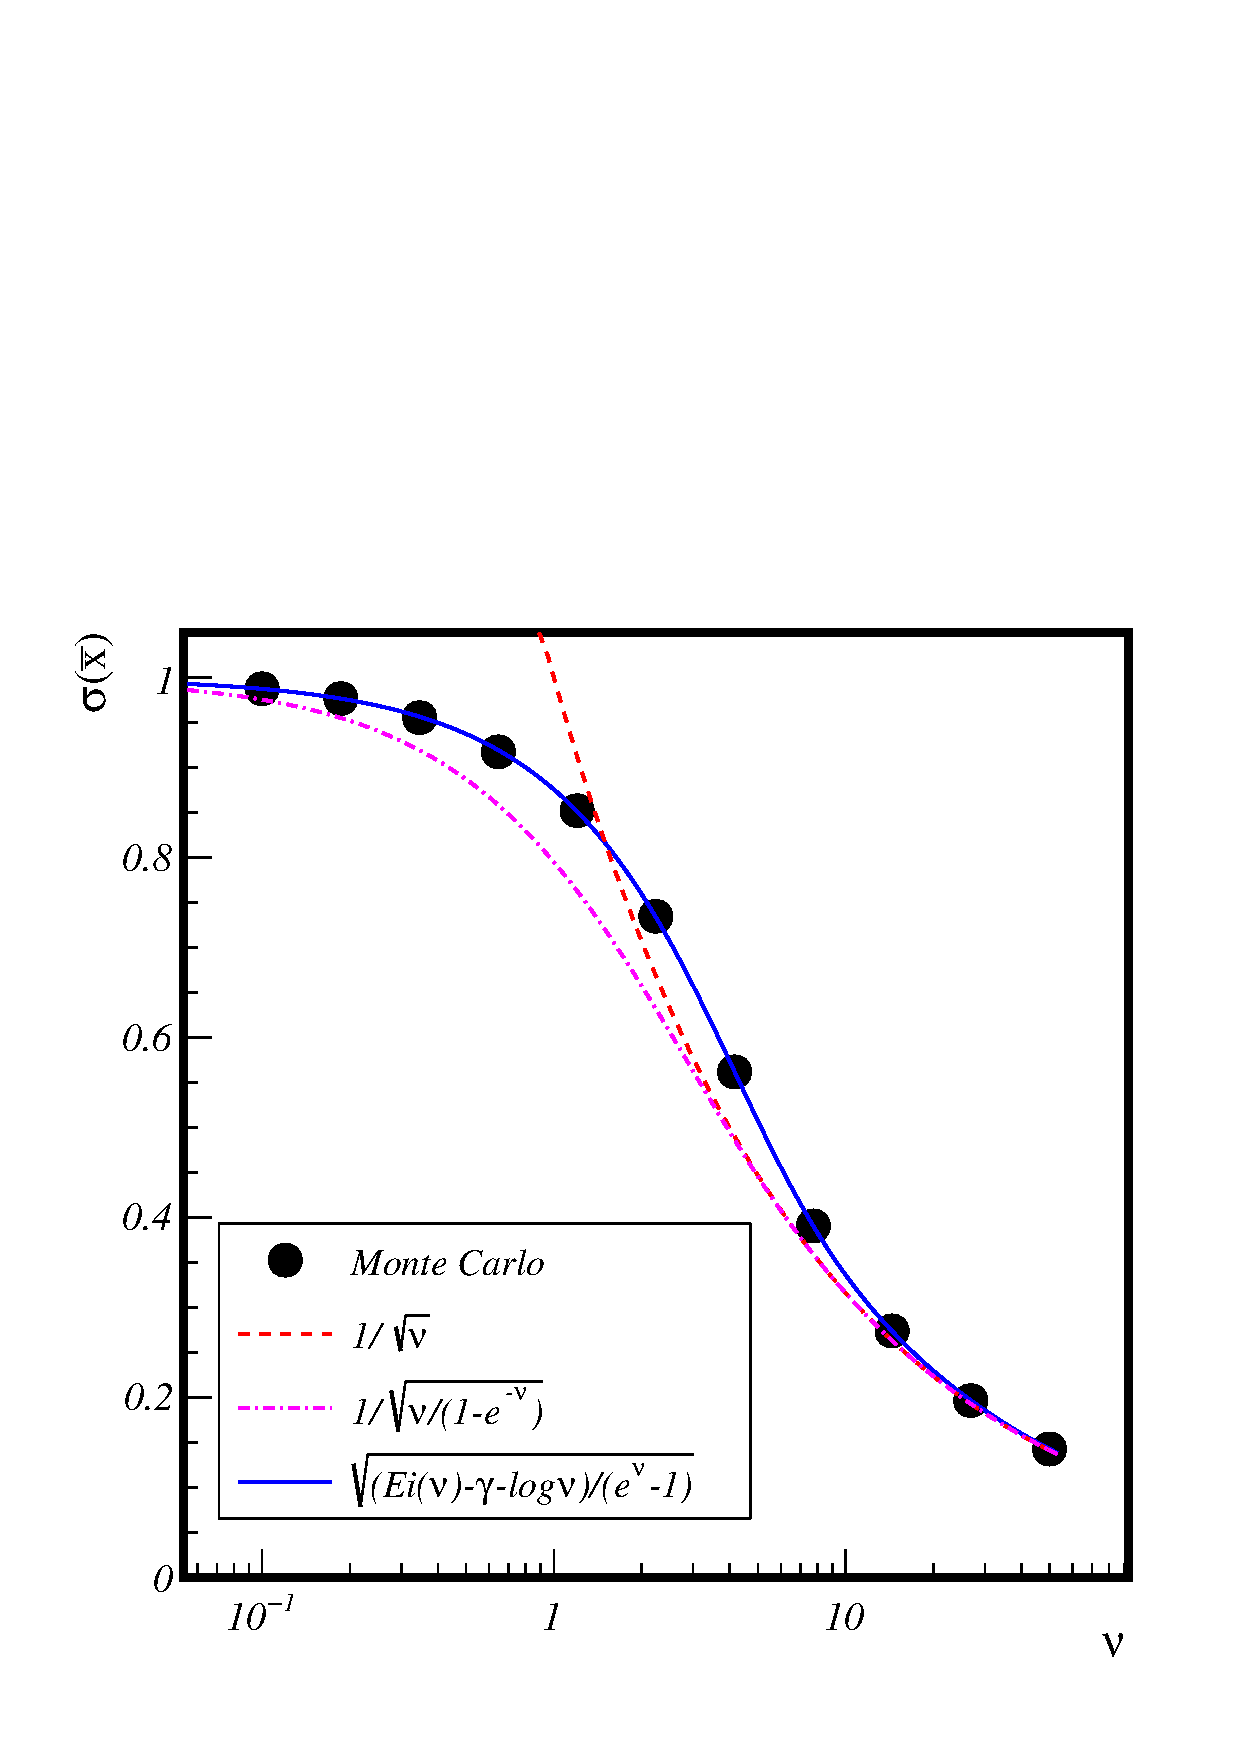
\includegraphics[width=0.6\textheight]{sigmean.pdf}
\caption{\small Зависимость ошибки средней величины в зависимости от среднего числа измерений для разных методов оценки: кружками показана оценка 
методом Монте-Карло, линиями -- разные функции от $\nu$.}
\label{fig:sigmean}
\end{center}
\end{figure}

Как видно, оценка ошибки среднего радиуса по формуле (\ref{eq:sigmean}) дает наиболее близкое значение к результатам, полученным по методу Монте-Карло. 
Эта оценка будет использоваться в дальнейшем.

\subsection{Программа FARICHRES}
Программа FARICHRES оптимизирует распределение черенковских фотонов в детекторе 
черенковских колец с фокусирующим аэрогелевым радиатором ФАРИЧ и в результате выдает описание оптимального радиатора,
вычисленное однофотонное распределенея по радиусу кольца и ошибки по углу и радиусу. 
Программа написана на языке {\em C++} под операционную систему {\em Linux}, использует пакет 
физического анализа {\em ROOT} \cite{root} и библиотеку {\em GSL} \cite{gsl}.
Исходные файлы программы и описание опубликованы на ресурсе GitHub:\\
\url{https://github.com/skononov/farich.git}.

Справка по использованию программы FARICHRES:
{\small
\begin{verbatim}
Usage: ./farichres [OPTIONS] qefile
Вычисляет разрешение детектора черенковских колец с многослойным фокусирующим аэрогелем.
Оптимизирует разрешение. Параметр qefile задает путь к файлу с данными о квантовой
эффективности фотонного детектора, представленых в двух колонках: 
длина волны (нм), эффективность (%).

 OPTIONS:
   -q                Задачный режим без графики и интерпретатора
   -e eff            Фактор к эффективности фотонного детектора, 0<eff<=1 
                     (по умолчанию: 1)
   -p size           Размер квадратного пикселя фотонного детектора, мм 
                     (по умолчанию: 0)
   -D distance       Расстояние от начала радиатора до фотонного детектора, мм 
                     (по умолчанию: 100)
   -n ri1            Максимальный показатель преломления радиатора на 400 нм 
                     (по умолчанию: 1.07)
   -i filename       Прочитать описание радиатора из текстового файла filename с колонками:
                     толщина слоя (мм), показатель преломления на 400 нм,
                     начиная с первого слоя (по умолчанию: оптимизированный радиатор)
   -N nlayers        Число слоев аэрогеля, 0<nlayers<=100 (по умолчанию: 3)
   -T thickness      Толщина радиатора, мм (по умолчанию: 25)
   -s Lsc            Длина рассеяния на 400 нм, мм (по умолчанию: 50)
   -b beta           Оптимизировать радиатор для данной скорости частицы, 1/ri1<beta<=1
                     (по умолчанию: 1)
   -B beta           Сделать расчет для данной скорости частицы, 1/ri1<beta<=1 
                     (по умолчанию: скорость частицы для оптимизации)
   -m[param]         Оптимизировать радиатор по угловой ошибке на трек, 
                     используя параметризацию param:
                     nt, pol<k>[s] (k=1..10, s - одинаковая толщина слоев) 
                     (по умолчанию: nt)
   -o filename       Сохранить гистограмму распределения по радиусу в заданный 
                     ROOT-файл filename (по умолчанию: farichres.root)
   -O filename       Сохранить описание детектора в командный файл Geant4 filename.
                     (по умолчанию: не cохранять).
\end{verbatim}
}

Радиатор может задаваться программе двумя разными способами:
\begin{description}
 \item[Способ с заданным профилем показателя преломления:] текстовый файл с описанием аэрогелевого радиатора 
      (опция {\tt -i filename}) с двумя значениями в строке, разделенных пробелами: 
      \begin{enumerate}
        \item[1)] толщина слоя в мм, начиная с ближайшего к фотодетектору;
        \item[2)] показатель преломления слоя при 400 нм.
      \end{enumerate}
 \item[Способ с быстрой оптимизацией:] число слоев $N$ (опция {\tt -N nlayers}) с суммарной толщиной $T$ (опция {\tt -T thickness}) и показателем преломления 
      в {\em первом} (ближайшем к фотодетектору) слое радиатора $n_1$ (опция {\tt -n ri1});
\end{description}
Расстояние $D$ от входной поверхности радиатора (дальней от фотодетектора) до входного окна фотодетектора задается опцией {\tt -D distance}.
Длина рэлеевского рассеяния света в аэрогеле \lsc при длине волны 400\,нм задается опцией {\tt -s Lsc}. 
Скорость частицы \betaop в единицах скорости света вакууме, для которой оптимизируется радиатор, задается опцией {\tt -b beta}. 
Можно также задать скорость частицы $\beta$, для которой производится финальный расчет разрешения, опцией {\tt -B beta}.
Эффективность фотонного детектора в зависимости от длины волны задается текстовым файлом в качестве обязательного аргумента программы. 
Эту эффективность можно уменьшить, задав коэффициент $\varepsilon$ опцией {\tt -e eff}, учитывая таким образом иные источники потерь черенковского света. 
Размер стороны квадратного пикселя фотодетектора $a$ задается опцией {\tt -p size}. Результат расчета радиатора в виде гистограмм и дерева записывается 
в ROOT-файл, заданный опцией {\tt -o filename}. Также с помощью опции {\tt -O filename} можно сохранить описание радиатора в формате макроса Geant4 
для программы моделирования ФАРИЧ.

В качестве результата программа выдает гистограмму распределения фотонов по радиусу кольца без учета координатного разрешения фотодетектора, гистограмму
распределения показателя по слоям аэрогеля, а также рассчитанные ошибки радиуса и черенковского угла на один фотон и на трек. 
Дополнительно рассчитываются ошибки, учитывающие вклад координатного разрешения 
фотодетектора, для этого к однофотонной ошибке по радиусу квадратично добавляется величина $\frac{a}{\sqrt{12}}$.

Перед расчетом радиатор оптимизируется с помощью быстрого метода, который описан ниже в разделе~\ref{ss:defopt}.

Численный расчет распределения фотонов по радиусу кольца происходит посредством разбиения диапазона длин волн и интервала 
радиусов на большое число (порядка 100) малых отрезков. Далее, для каждого отрезка по длине волны и каждого отрезка по радиусу находятся 
все точки излучения фотонов в радиаторе. Интеграл (\ref{eq:dnpedr}) заменяется на сумму по длинам волн и точкам излучения.
При этом производные $\frac{\partial R}{\partial x}$ приблизительно заменяются на $\frac{\Delta R}{\Delta x}$, где $\Delta x$ --- отрезок пути частицы 
в слое радиатора, дающий вклад в интервал радиусов $\Delta R$.

Если указана опция {\tt -m[param]}, проводится численная минимизация ошибки черенковского угла на трек (без учета вклада пикселя) 
методом Migrad библиотеки {\em Minuit2} \cite{minuit2}, входящей в пакет анализа {\em ROOT}. Методы библиотеки {\em Minuit2} не 
позволяют выполнить условную минимизацию, которая требуется для фиксированной полной толщины радиатора. 
Для применения {\em Minuit2} требуется переопределить параметры так, чтобы их можно было варьировать независимо друг от друга.
Реализованы два варианта параметризации толщин и показателей преломления слоев:
\begin{enumerate}
\item NT-параметризация (опция {\tt -mnt}), см. разд.~\ref{ss:ntpar};
\item полиномиальная параметризация (опция {\tt -mpol$k$}, $k=1\ldots 10$), см. разд.~\ref{ss:polpar}.
\end{enumerate}
По умолчанию, когда в параметризации не задан (опция {\tt -m}), используется NT-параметризация.
Во всех вариантах оптимизации фиксированы показатель преломления первого слоя $n_1$, полная толщина радиатора $T$, число слоев аэрогеля $N$.

\subsection{Быстрая оптимизация радиатора}
\label{ss:defopt}
В этом варианте не используется расчет разрешения ФАРИЧ по углу, а оптимизация происходит из условия, чтобы границы изображений колец от каждого слоя при 
некоторой длине волны $\lambda_0$ совпадали. Длина волны выбирается соответствующей максимуму спектра регистрируемых не рассеянных фотонов.
Условие совпадения колец можно выразить в виде следующей системы нелинейных уравнений на толщины и показатели преломления слоев $t_i,\,n_i, i=1\ldots N$ для заданных
параметров первого слоя $t_1,\,n_1$ для длины волны $\lambda_0$:
\begin{align}\label{eq:defopt}
t_0 U_{10} & = t_0 U_{20} + t_1 U_{21},              & t_2 U_{22} & = t_1 U_{11}, \nonumber\\
t_0 U_{10} & = t_0 U_{30} + t_1 U_{31} + t_2 U_{32}, & t_3 U_{33} & = t_1 U_{11}, \nonumber\\
& \ldots, & & \ldots, \\
t_0 U_{10} & = t_0 U_{N0} + t_1 U_{N1} + t_2 U_{N2} + \ldots + t_{N-1} U_{N(N-1)}, & t_N U_{NN} & = t_1 U_{11}, \nonumber
\end{align}
где $t_0=D-T$ -- ширина воздушного зазора между радиатором и фотонным детектором, $U_{kl} = \tan\psi_{kl}$ -- тангенс угла черенковского излучения $k$-го слоя в $i$-ом слое
согласно выражению (\ref{eq:tanpsi}). Левая колонка уравнений в (\ref{eq:defopt}) выражает равенства радиусов внутренней границы колец для всех слоев, правая колонка --- равенства
ширин колец. При этом первый ряд уравнений соответствует второму слою, второй ряд -- третьему и т.д. Решение системы уравнений (\ref{eq:defopt}) происходит последовательно 
сверху внизу, слева направо. Сначала методом итераций решается левое уравнение в ряду относительно показателя преломления слоя, затем из правого уравнения находится толщина слоя.

Можно заметить, что суммарная толщина радиатора при этом получается больше, чем заданная. Чтобы достичь заданную толщину радиатора, система уравнений решается повторно методом итераций: толщина первого слоя в нулевом приближении задается равной $t_1^0 = T/N$, 
для $i$-ой итерации ($i\geq 1$) толщина первого слоя равна $t_1^i=t_1^{i-1} T/T^{i-1},$ $T^{i-1}$ -- суммарная толщина радиатора, полученная на $i-1$ итерации. 
Итерации продолжаются пока не будет достигнута требуемая относительная точность на полную толщину радиатора.

Быстрый метод позволяет оптимизировать радиатор с любым числом слоев быстрее, чем методы основанные на вычислении углового разрешения, при этом давая близкое 
итоговое угловое разрешение.

\subsection{NT-параметризация}
\label{ss:ntpar}
Можно определить невырожденную матрицу преобразования вектора толщин слоев $\boldsymbol{t}=(t_1,t_2,\ldots\,,t_{N})$ в вектор 
специальных параметров $\boldsymbol{u}=(u_1,u_2,\ldots,u_{N})$, в котором полная толщина задается одним параметром, 
а остальные определяют подпространство значений толщин $\boldsymbol{t}$, в котором полная толщина неизменна. 
Ортогональную матрицу такого преобразования можно получить с помощью сингулярного 
разложения однострочной матрицы $1\times N$ $M=(1,1,\ldots,1)$, являющейся матрицей коэффициентов линейного уравнения:
\begin{equation}
t_1+t_2+\ldots+t_{N} = T.
\label{eq:totthick}
\end{equation}
В результате данного разложения матрица $M$ представляется в виде произведения трех матриц $M=U\Sigma V^T$, где $U=1\, \mathrm{или}\, -1$,
$V^T$ --- искомая ортогональная матрица $N\times N$, а $\Sigma$ --- матрица $1\times N$ с положительным первым элементом (сингулярным числом матрицы $M$) и остальными 
нулевыми элементами. Вектор $\boldsymbol{u} = V^T \boldsymbol{t}$ также определяет толщины всех слоев радиатора, при этом первый элемент $u_1$ задает полную толщину. 
Можно сказать, что $V^T$ является матрицей перехода в  базис векторного пространства, в котором первый базисный вектор нормален гиперплоскости, задаваемой уравнением (\ref{eq:totthick}).

Сингулярное разложение выполняется с помощью класса {\em TDecompSVD} пакета {\em ROOT}. В силу того, что {\em TDecompSVD} требует, чтобы разлагаемая матрица 
имела число строк не менее, чем число столбцов, матрица $M$ преобразуется в квадратную добавлением $N-1$ нулевых строк, что не влияет на свойства ортогональной матрицы $V$.

Свободными параметрами минимизации являются $N-1$ показателей преломления слоев $n_i, i=2\ldots N$ и $N-1$ параметров $u_i, i=2\ldots N$. 
Полное число свободных параметров равно $2\,N - 2$.

Метод оптимизации с использованием NT-параметризации далее для краткости называется NT-оптимизацией.

\subsection{Полиномиальная параметризация}
\label{ss:polpar}
В этом варианте распределение показателя преломления по толщине радиатора описывается с помощью значений многочлена степени $k$ в серединах 
слоев радиатора. При этом толщины слоев можно выбрать одинаковыми (опция {\tt -mpol<k>s}), либо использовать толщины, полученные методом быстрой 
оптимизации (опция {\tt -mpol<k>}).

Многочлен задается выражением
\[ Q_k(x) = n_1 + C_1(x-x_1) + C_2(x-x_1)^2 + \ldots + C_k(x-x_1)^k, \]
где $n_1,\,x_1$ -- значения показателя преломления и координата $x$ середины первого слоя. Показатели преломления слоев соответственно равны
\[ n_i = Q_k(x_i), i=1\ldots N. \]
Свободными параметрами минимизации являются коэффициенты многочлена $C_1$, $C_2$, \ldots, $C_k$. Поскольку в данном методе число 
свободных параметров равно $k$, которое можно взять небольшим в практически важных случаях, то вычислительная сложность минимизации 
не зависит от числа слоев, как в случае NT-оптимизации. В программе FARICHRES можно задать вплоть до 100 слоев для полиномиальной оптимизации. 
Преимущество полиномиальной параметризации в том, что она позволяет оптимизировать радиатор с практически непрерывным изменением показателя преломления по толщине.

Для надежной сходимости процедуры минимизации необходимо достаточно точно определить начальные значения
параметров и начальные шаги по ним. Для этого производится линейная подгонка параметров многочлена $Q_k$ к распределению показателя преломления,
полученному с быстрой оптимизацией. Размер шага выбирается равным 0,01 от найденного абсолютного значения параметра.

Для описания распределения показателя преломления аэрогеля с любым числом слоев достаточно многочлена второй степени $Q_2(x)$, имеющего два свободных параметра. 
При дальнейшем увеличении степени многочлена угловое разрешение для оптимизированного радиатора изменяется незначительно.

Вариант оптимизации с использованием полиномиальной параметризации с многочленом второй степени и толщинами слоев, полученными из быстрой 
оптимизации, далее называется Pol2-оптимизация.

\section{Результаты расчета}
Ниже, если не указано иное, производится расчет для фотодетектора в виде квадратного массива кремниевых фотоумножителей 
MPPC 14161-3050HS с коэффициентом эффективности $\varepsilon=0.82$ и размером пикселя $a=3$\,мм. 
Показатель преломления в первом слое $n_1=1.05$, расстояние между радиатором и фотонным детектором составляет $D=200$\,мм, полная толщина радиатора $T=40$\,мм, 
скорость частицы для оптимизации и расчета $\beta=1$.

\subsection{Сравнение методов оптимизации радиатора}
Проведен расчет распределения по радиусу и разрешения для радиатора с 4 слоями, оптимизированный разными методами. Разрешение по углу для одного фотона 
$\sigma_1(\theta)$ и для частицы $\sigma_t(\theta)$ без учета вклада размера пикселя представлено в таблице \ref{tab:methcomp}. 

\begin{table}[htbp]
\caption{Число фотоэлектронов и угловое разрешение (без учета пикселя) для разных методов оптимизации радиатора ФАРИЧ.}
\label{tab:methcomp}
\begin{center}
\begin{tabular}{lcccc}\hline
Метод оптимизации   & $N_\mathrm{pe}$ & $R$, мм & $\sigma_1(\theta)$, мрад & $\sigma_t(\theta)$, мрад \\\hline
Быстрая оптимизация & 68,8 & 55,32 & 5,01 & 0,608 \\\hline
NT-оптимизация      & 68,7 & 55,28 & 4,96 & 0,603 \\\hline
Pol2-оптимизация    & 69,0 & 55,42 & 5,00 & 0,606 \\\hline
\end{tabular}
\end{center}
\end{table}

На рисунке~\ref{fig:methcomp} показаны однофотонные распределения по радиусу в плоскости фотодетектора (без учета размера пикселя) 
для разных вариантов оптимизации. 
\begin{figure}[htbp]
\begin{center}
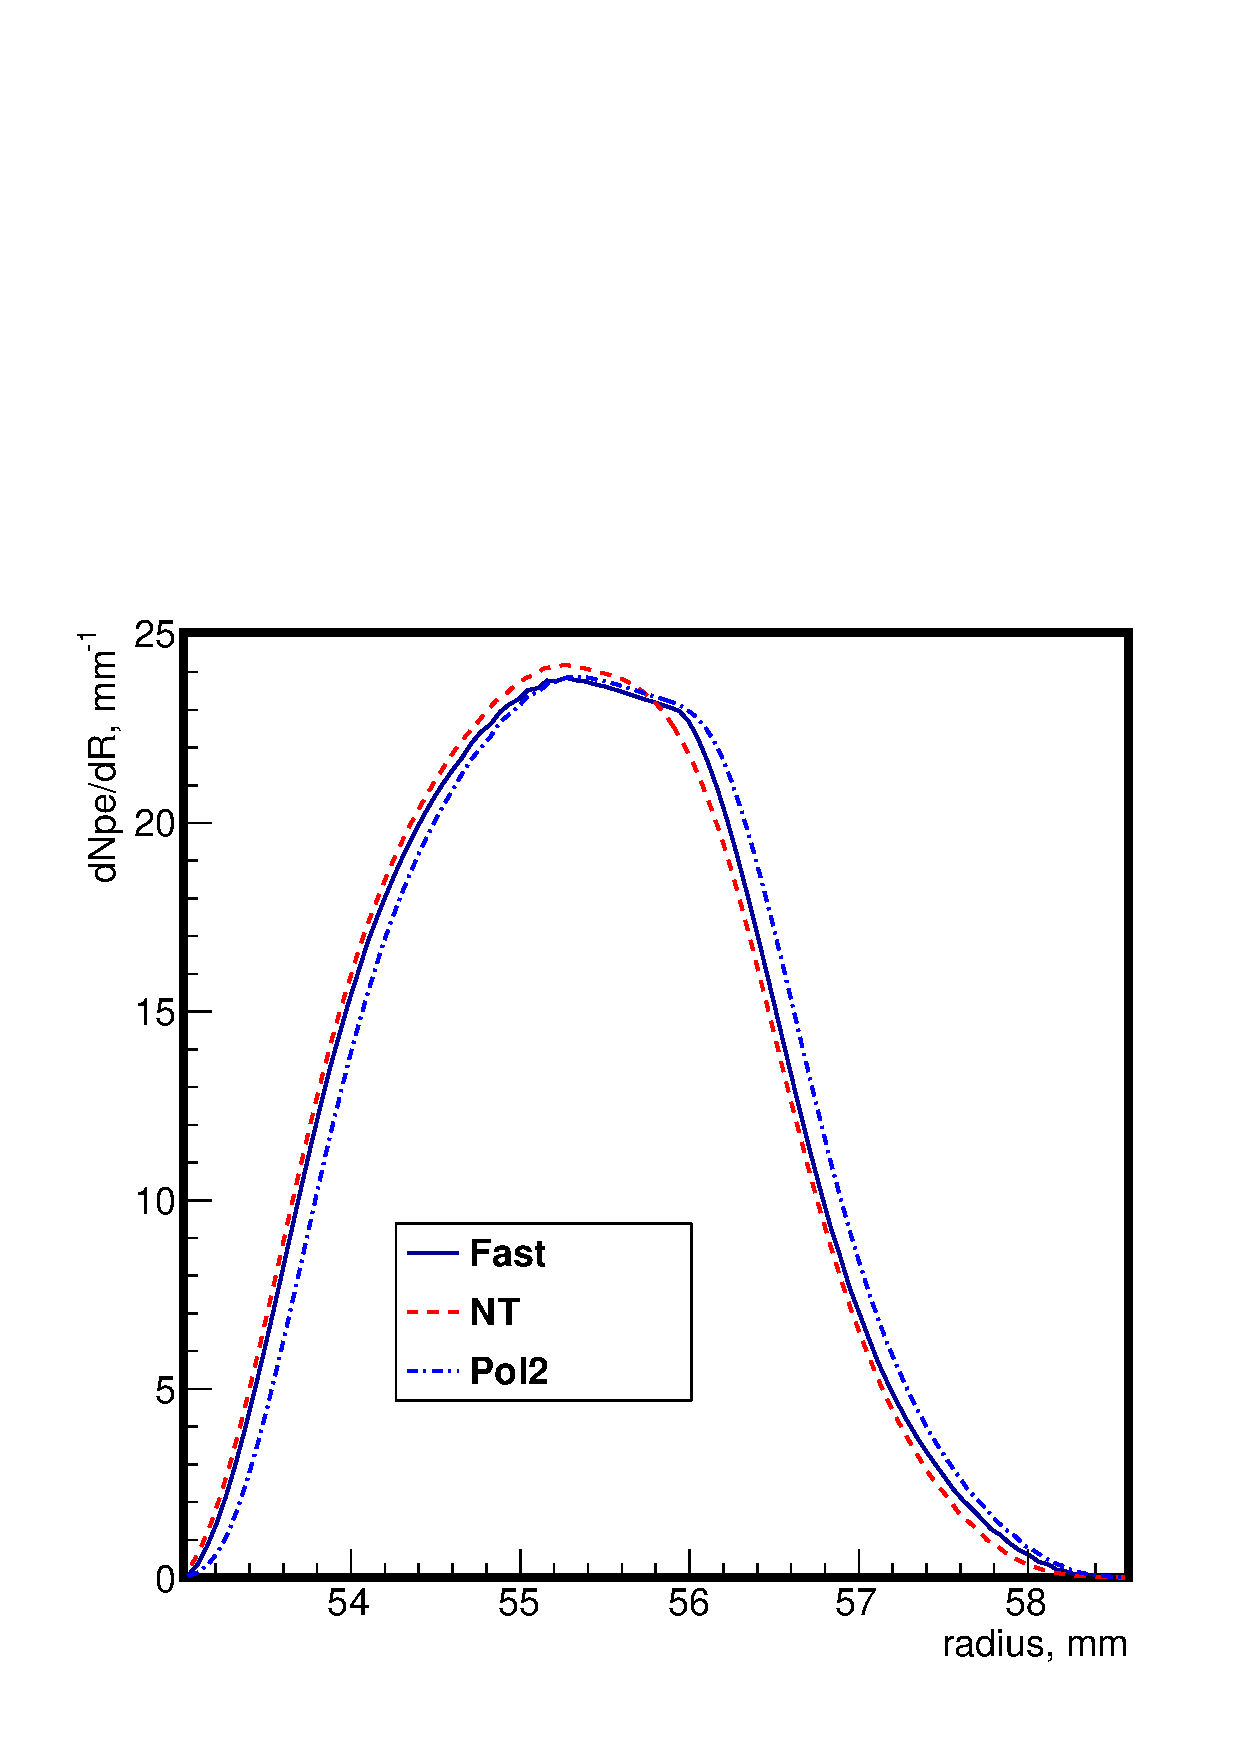
\includegraphics[width=0.8\textwidth]{hrad_mla4_varopt.pdf}
\caption{Распределения фотонов по радиусу для трех вариантов оптимизации радиатора.}
\label{fig:methcomp}
\end{center}
\end{figure}

Результаты сравнения показывают, что в рассмотренной конфигурации ФАРИЧ быстрая оптимизация дает угловое разрешение лишь на 1\% хуже чем NT-оптимизация. 
Разница между быстрой и Pol2-оптимизацией в угловом разрешении еще меньше --- 0,2--0,3\%. Разница между методами в угловом разрешении будет в два 
раза меньше, если учесть вклад размера пикселя. Если взять в два раза меньшее расстояние между радиатором и фотонным детектором -- 100\,мм, 
то разница между быстрым методом и NT-методом возрастает, но только до 1,5\%.

На рисунке~\ref{fig:layersmethcomp}(a) показана зависимость углового разрешения на частицу 
для оптимизированных разными методами радиаторов в зависимости от числа слоев. Рисунок~\ref{fig:layersmethcomp}(b) показывает
относительную разницу в разрешении для радиаторов, оптимизированных разными методами.
В силу сложности вычислений NT-оптимизация применялась только для числа слоев не более 10. Впрочем, видно, что угловое разрешение
незначительно меняется для числа слоев более 10.
\begin{figure}[htbp]
\begin{center}
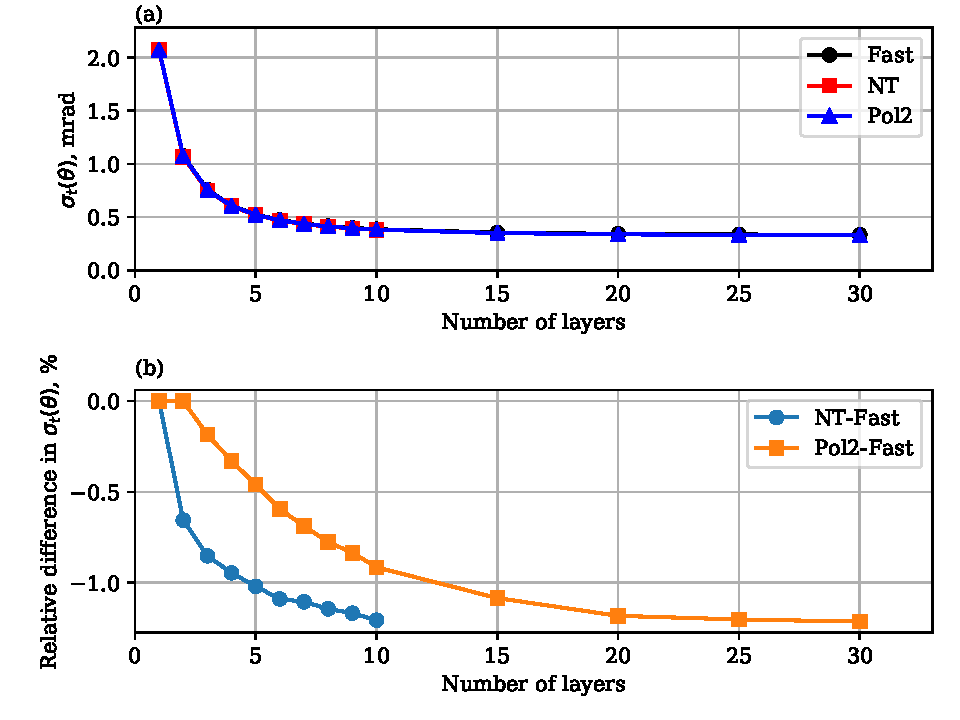
\includegraphics[width=0.8\textwidth]{sigtang_vs_layers_varopt.pdf}
\caption{(a) Ошибка угла на частицу в зависимости от количества слоев радиатора для трех вариантов оптимизации. 
(b) Относительная разница угловых ошибок на частицу для разных методов оптимизации.}
\label{fig:layersmethcomp}
\end{center}
\end{figure}

Таким образом, можно сделать вывод, что быстрый метод оптимизации дает решение близкое к оптимальному и может быть использован для практически всех случаев.

\subsection{Разрешение ФАРИЧ в зависимости от числа слоев}

На рисунке~\ref{fig:hradlayers} показаны распределения фотонов по радиусу кольца для разного числа слоев. Радиатор получен с помощью Pol2-оптимизации.
\begin{figure}[htbp]
\begin{center}
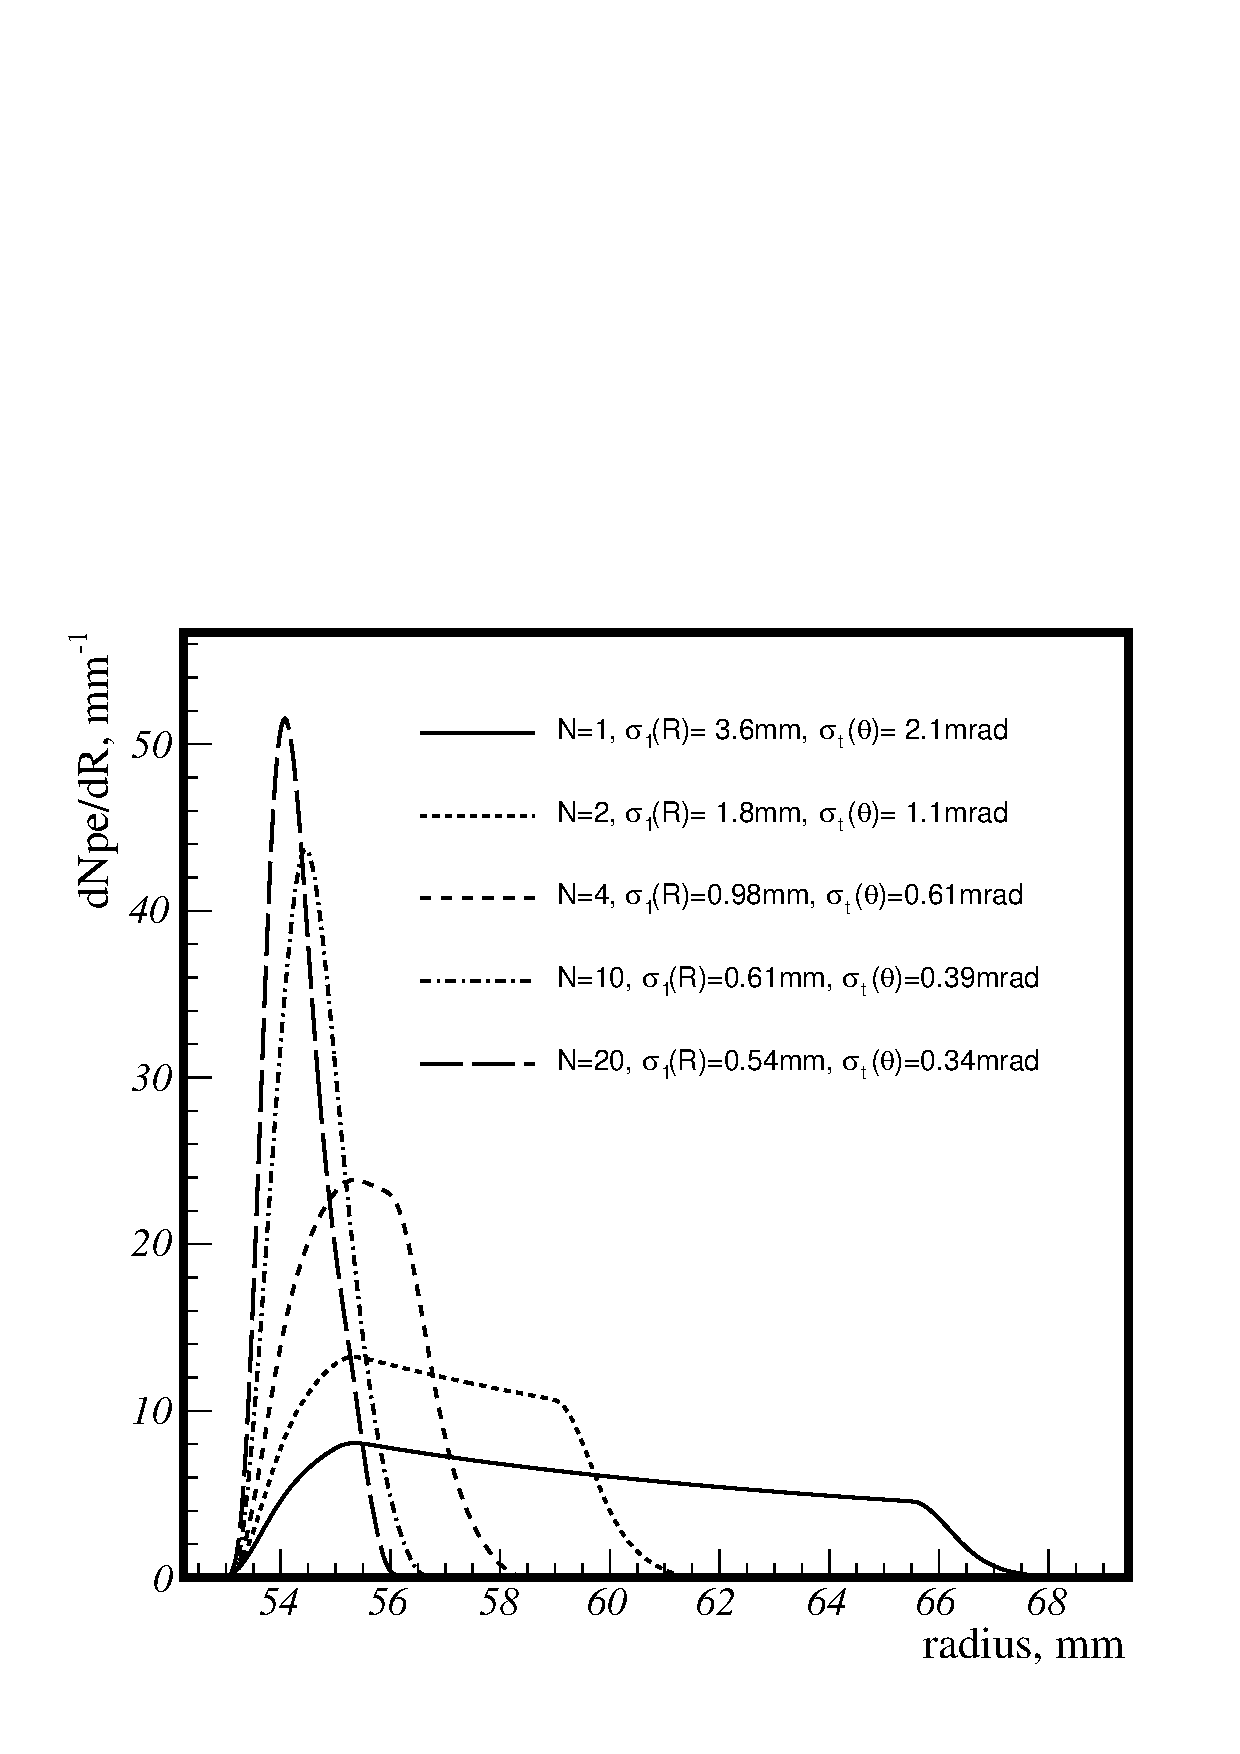
\includegraphics[width=0.6\textwidth]{hrad_varlayers_pol2opt.pdf}
\caption{Распределение фотоэлектронов по радиусу кольца для разного числа слоев радиатора, полученного с помощью Pol2-оптимизации. 
В легенде указано число слоев $N$, однофотонное разрешение по радиусу $\sigma_1(R)$ и угловое разрешение на частицу $\sigma_t(\theta)$.}
\label{fig:hradlayers}
\end{center}
\end{figure}

\begin{table}[htbp]
\caption{Параметры детектора ФАРИЧ для разного числа слоев радиатора.}
\label{tab:parlayers}
\begin{center}
\begin{tabular}{lccccc}\hline
Число слоев &  1 &  2 &  4 & 10 & 20\\\hline
$N_\mathrm{pe}$ &   77 &   72 &   69 &   67 &   67\\\hline
$R$, мм &  59.5 &  56.8 &  55.4 &  54.6 &  54.3\\\hline
\multicolumn{6}{c}{Ошибки без учета размера пикселя}\\\hline
$\sigma_1(R)$, мм &  3.6 &  1.8 & 0.99 & 0.62 & 0.54\\\hline
$\sigma_t(R)$, мм & 0.41 & 0.21 & 0.12 & 0.076 & 0.067\\\hline
$\sigma_1(\theta)$, мрад &   18 &    9 &    5 &  3.1 &  2.8\\\hline
$\sigma_t(\theta)$, мрад &  2.1 &  1.1 & 0.61 & 0.39 & 0.34\\\hline
\multicolumn{6}{c}{Ошибки с учетом размера пикселя}\\\hline
$\sigma_1(R)$, мм &  3.7 &    2 &  1.3 &  1.1 &    1\\\hline
$\sigma_t(R)$, мм & 0.43 & 0.24 & 0.16 & 0.13 & 0.13\\\hline
$\sigma_1(\theta)$, мрад &   19 &   10 &  6.7 &  5.4 &  5.2\\\hline
$\sigma_t(\theta)$, мрад &  2.1 &  1.2 & 0.81 & 0.67 & 0.64\\\hline
\end{tabular}
\end{center}
\end{table}


\section{Сравнение результатов расчета с моделированием в Geant4}
TODO

\begin{thebibliography}{99}
\bibitem{prudn} Прудников А. П., Брычков Ю. А., Маричев О. И. Интегралы и ряды. — Изд. 2-е. — М.: ФИЗМАТЛИТ, 2003. — Т. 1. — С. 320. — ISBN 5-9221-0323-7.
\bibitem{root} Пакет анализа ROOT [\url{https://root.cern.ch/}]
\bibitem{gsl} GNU Scientific Library [\url{http://www.gnu.org/software/gsl/}]
\bibitem{aerdisp} T. Bellunato et al., ``Refractive index dispersion law of silica aerogel'',
European Physics Journal C 52 (2007) 759-764
\bibitem{aerscat} A.F. Danilyuk et al., ``Recent results on aerogel development for use in Cherenkov counters'',
Nuclear Instruments and Methods in Physics Research A 494 (2002) 491–494
\bibitem{minuit2} Minuit2 User Guide [\url{https://root.cern.ch/root/htmldoc/guides/minuit2/Minuit2.html}]
\end{thebibliography}

\end{document}
